\section{Versuchsaufbau/-durchführung}
Der verwendete Aufbau ist in Abbildung~\ref{fig: aufbau} einzusehen. Bevor relevante Merkmale des Lasers vermessen werden können, ist eine
Justage des Aufbaus notwendig. Hierzu wird ein weiterer Laser und zwei Lochblenden verwendet. Am Laserrohr wird eine Hochspanung
angelegt, die die notwendige Gasentladung hervorruft. Durch Justierschrauben an den konfokalen Resonatorspiegeln (Radius jeweils $\SI{1.4}{\meter}$)
und dem Laserrohr werden die Elemente so eingestellt, dass die optischen Achsen aufeinander liegen und der Laser anfängt zu leuchten.
Zur Intensitätsmessung wird eine Photodiode verwendet, die hinter dem Laser positioniert ist.
\begin{figure}
  \centering
  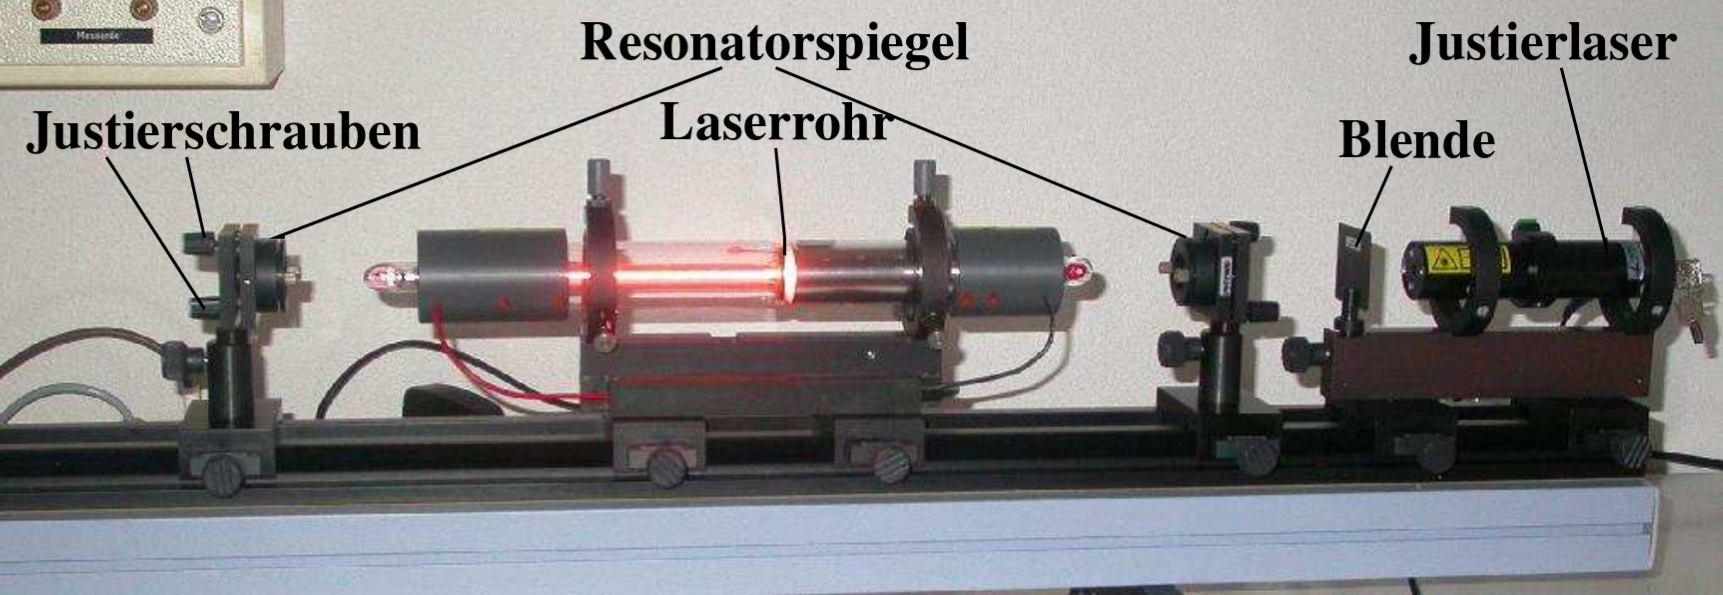
\includegraphics[width = 0.7\textwidth]{theorie_bilder/aufbau.png}
  \caption{Darstellung des verwendeten Aufbaus \cite{anleitung61}.}
  \label{fig: aufbau}
\end{figure}

Mittels der Interferenz an einem optischen Gitter soll die Wellenlänge des erzeugten Laserstrahls bestimmt werden. Hierzu werden das Gitter
und ein Schirm hinter dem Laser positioniert. Aus einer Messung des Abstandes zwischen Schirm und Gitter, sowie den auftretenden Intensitätsmaxima
auf dem Schirm kann die Wellenlänge berechnet werden
\begin{equation}
  \lambda = \frac{g \cdot \sin\left\{\arctan\left(\frac{d_n}{L} \right)  \right\}}{n},\quad n \in \mathbb{N}.
  \label{eq: interferenz}
\end{equation}
Mit der Gitterkonstanten $g$, dem Abstand des $n$-ten Interferentmaximums zum Hauptmaximum $d_{n}$ und dem Abstand zwichen Schirm und Gitter $L$.

Zur Untersuchung der TEM-Moden wird eine defokussierende Linse hinter den Laser gestellt, die den Laserstrahl verbreitert.
Mittels einer Mikrometerschraube kann die Photodiode
senkrecht zur Strahlachse verschoben werden und somit die Abhängigkeit zwischen Intensität und Achsenabstand untersucht werden. Zunächst
wird die Grundmode untersucht, die ohne Einsatz von Blenden gegenüber anderen Moden dominiert. Anschließeden wird die $I\ua{01}$-Mode
vermessen, welche eine Nullstelle bei $r = 0$ besitzt. Innherhalb des Resonators wird ein Wolframdraht so positioniert, dass die Grundmode
unterdrückt wird. Anschließend kann die $I\ua{01}$-Mode analog mit der Photodiode ausgemessen werden.

An den Ausgängen des Laserrohrs sind Brewster-Fenster angebracht. Hierbei handelt es sich um gläserne Platten, die
im Brewsterwinkel zu optischen Achse eingestellt werden. Gemäß den Fresnelschen Gleichungen ist der Brewsterwinkel jener Winkel, unter dem
die zur Einfallsebene parallele Komponente des elektrischen Lichtfeldes nicht reflektiert wird. Die senkrechte Komponente wird somit
durch Refelxion stark unterdrückt und das Licht linear polarisiert. Diese Gegebenheit soll
experimentell untersucht werden. Hinter den Laser wird hierzu ein drehbarer Polarisationsfilter platziert. In Abhängigkeit zum eingestellten Winkel
wird der Photostrom gemessen. Nach Malus ist die Intensität der linear polarisierten Lichtwelle hinter dem Polarisationsfilter
durch folgende Funktion zu beschreiben
\begin{equation}
  I(\varphi) = I\ua{0} \sin^2\left(\varphi + \varphi_0\right).
  \label{eq: malus}
\end{equation}
Mit den konstanten Parametern $I\ua{0}$ und $\varphi_0$ und dem relativ zu einer beliebigen Startachse eingestellten Winkel $\varphi$.

Abschließend soll die Stabilitätsbedingung \eqref{eq: stabilität} für
einen gekrümmten Spiegel $r = \SI{1.4}{\meter}$ und einen ebenen Spiegel quantitativ untersucht werden. Unter variabler Resonatorlänge $L$ wird hierzu der
Photostrom aufgezeichnet. Hierbei ist es notwendig bei jedem Abstand den Laser neu zu justieren und den Photostrom zu maximieren.
